\DocumentMetadata{%
 %  uncompress, %only for debugging!!
  pdfversion=2.0,
  testphase={phase-II, tabular, graphic}%
 % testphase={phase-II,math, tabular, graphic}% TOC Does not work
   % testphase={phase-III,math}% TOC works
}
\tagpdfsetup{activate, tabsorder=structure}
% Use the following to fix bug in November 2023 download of LaTeX
\ExplSyntaxOn
\cs_generate_variant:Nn\__tag_prop_gput:Nnn{cnx}
\ExplSyntaxOff
\documentclass[11pt,
  english,
  letterpaper,
]{article}
\usepackage{sa4ss}
\usepackage{amsmath,amssymb,array}
\usepackage{booktabs}

% From tagged-template.latex
\usepackage{lmodern}
\usepackage{ifxetex,ifluatex}
\ifnum 0\ifxetex 1\fi\ifluatex 1\fi=0 % if pdftex
  \usepackage[T1]{fontenc}
  \usepackage[utf8]{inputenc}
  \usepackage{textcomp} % provide euro and other symbols
\else % if luatex or xetex
  \usepackage{unicode-math}
  \defaultfontfeatures{Scale=MatchLowercase}
  \defaultfontfeatures[\rmfamily]{Ligatures=TeX,Scale=1}
\fi

% Use upquote if available, for straight quotes in verbatim environments
\IfFileExists{upquote.sty}{\usepackage{upquote}}{}
\IfFileExists{microtype.sty}{% use microtype if available
  \usepackage[]{microtype}
  \UseMicrotypeSet[protrusion]{basicmath} % disable protrusion for tt fonts
}{}
\makeatletter
\@ifundefined{KOMAClassName}{% if non-KOMA class
  \IfFileExists{parskip.sty}{%
    \usepackage{parskip}
  }{% else
    \setlength{\parindent}{0pt}
    \setlength{\parskip}{6pt plus 2pt minus 1pt}}
}{% if KOMA class
  \KOMAoptions{parskip=half}}
\makeatother
\usepackage{xcolor}
\IfFileExists{xurl.sty}{\usepackage{xurl}}{} % add URL line breaks if available
\hypersetup{
  pdflang={en},
  hidelinks,
  pdfcreator={LaTeX via pandoc}}
\urlstyle{same} % disable monospaced font for URLs
\usepackage{longtable}
% Correct order of tables after \paragraph or \subparagraph
\usepackage{etoolbox}
\makeatletter
\patchcmd\longtable{\par}{\if@noskipsec\mbox{}\fi\par}{}{}
\makeatother
% Allow footnotes in longtable head/foot
\IfFileExists{footnotehyper.sty}{\usepackage{footnotehyper}}{\usepackage{footnote}}
\makesavenoteenv{longtable}
\usepackage{graphicx}
\makeatletter
\def\maxwidth{\ifdim\Gin@nat@width>\linewidth\linewidth\else\Gin@nat@width\fi}
\def\maxheight{\ifdim\Gin@nat@height>\textheight\textheight\else\Gin@nat@height\fi}
\makeatother
% Scale images if necessary, so that they will not overflow the page
% margins by default, and it is still possible to overwrite the defaults
% using explicit options in \includegraphics[width, height, ...]{}
\setkeys{Gin}{width=\maxwidth,height=\maxheight,keepaspectratio}
% Set default figure placement to htbp
\makeatletter
\def\fps@figure{htbp}
\makeatother
\setlength{\emergencystretch}{3em} % prevent overfull lines
\providecommand{\tightlist}{%
  \setlength{\itemsep}{0pt}\setlength{\parskip}{0pt}}
\setcounter{secnumdepth}{5}
\usepackage{lineno}
\usepackage[inline]{showlabels}
\usepackage{pdflscape}
\ifxetex
  % Load polyglossia as late as possible: uses bidi with RTL langages (e.g. Hebrew, Arabic)
  \usepackage{polyglossia}
  \setmainlanguage[]{}
\else
  \usepackage[shorthands=off,main=english]{babel}
\fi

%Define cslreferences environment, required by pandoc 2.8
%https://github.com/rstudio/rmarkdown/issues/1649
\newlength{\csllabelwidth}
\setlength{\csllabelwidth}{3em}
\newlength{\cslhangindent}
\setlength{\cslhangindent}{1.5em}
% for Pandoc 2.8 to 2.10.1
\newenvironment{cslreferences}%
  {}%
  {\par}
% For Pandoc 2.11+
\newenvironment{CSLReferences}[2] % #1 hanging-ident, #2 entry spacing
 {% don't indent paragraphs
  \setlength{\parindent}{0pt}
  % turn on hanging indent if param 1 is 1
  \ifodd #1 \everypar{\setlength{\hangindent}{\cslhangindent}}\ignorespaces\fi
  % set entry spacing
  \ifnum #2 > 0
  \setlength{\parskip}{#2\baselineskip}
  \fi
 }%
 {}
\usepackage{calc}  % for \widthof, \maxof in minipage
\newcommand{\CSLBlock}[1]{#1\hfill\break}
\newcommand{\CSLLeftMargin}[1]{\parbox[t]{\csllabelwidth}{#1}}
\newcommand{\CSLRightInline}[1]{\parbox[t]{\linewidth - \csllabelwidth}{#1}\break}
\newcommand{\CSLIndent}[1]{\hspace{\cslhangindent}#1}


\providecommand{\tightlist}{%
  \setlength{\itemsep}{0pt}\setlength{\parskip}{0pt}}

\usepackage{lineno}
\usepackage[inline]{showlabels}
\usepackage{pdflscape}
\date{}
\newcommand{\trTitle}{}
\newcommand{\trYear}{2023}
\newcommand{\trMonth}{May}
\newcommand{\trAuthsLong}{truetruetrue}
\newcommand{\trAuthsBack}{Monk, M.H., C.R. Wetzel, J. Coates}
\newcommand{\trCitation}{
\begin{hangparas}{1em}{1}
\trAuthsBack{}. \trYear{}. \trTitle{}. \glsentrylong{pfmc}, Portland, Oregon. \pageref{LastPage}{}\,p.
\end{hangparas}}

\newcommand\includegraphicsifexists[2][width=\linewidth]{\IfFileExists{#2}{\includegraphics[#1]{#2}}{}}

\begin{document}

%%%%% Frontmatter %%%%%

% Footnote symbols in front matter
\renewcommand*{\thefootnote}{\fnsymbol{footnote}}

\small
\thispagestyle{empty}
\pagenumbering{roman}
\noindent
\begin{center}
\title{}
% \textnormal{\MakeTextUppercase{\trTitle{}}}
\vspace{1.5cm}
{\Large\textbf\newline{}}

\includegraphicsifexists[width=4in]{figure_title.png}
\vfill
by\\
Melissa H. Monk\textsuperscript{1}\\
Chantel R. Wetzel\textsuperscript{2}\\
Julia Coates\textsuperscript{3}\vfill
\textsuperscript{1}Southwest Fisheries Science Center, U.S. Department of Commerce, National Oceanic and Atmospheric Administration, National Marine Fisheries Service, 110 McAllister Way, Santa Cruz, California 95060\\
\textsuperscript{2}Northwest Fisheries Science Center, U.S. Department of Commerce, National Oceanic and Atmospheric Administration, National Marine Fisheries Service, 2725 Montlake Boulevard East, Seattle, Washington 98112\\
\textsuperscript{3}California Department of Fish and Wildlife, Marine Region 1933 Cliff Drive, Suite 9, Santa Barbara, California 93109\vfill
\trMonth{} \trYear{}
\end{center}
\clearpage

% Fourth page: Colophon
\thispagestyle{empty}
\vspace*{\fill}
\begin{center}
\copyright{} \glsentrylong{pfmc}, \trYear{}\\
\end{center}
\par
\bigskip
\noindent
Correct citation for this publication:
\bigskip
\par
\trCitation{}
\clearpage

% Add TOC to pdf bookmarks (clickable pdf)
\pdfbookmark[1]{\contentsname}{toc}

% Table of contents page, lists of figures and tables
\tableofcontents\clearpage
\label{TRlastRoman}
\clearpage

% Table of contents
\newpage
\thispagestyle{empty} % to remove page number

% Settings for the main document
\pagenumbering{arabic}  % Regular page numbers
\pagestyle{plain}  % No page number on first page of main document, use 'empty'
\renewcommand*{\thefootnote}{\arabic{footnote}}  % Back to numeric footnotes
\setcounter{footnote}{0}  % And start at 1
\renewcommand{\headrulewidth}{0.5pt}
\renewcommand{\footrulewidth}{0.5pt}
%\pagestyle{fancy}\fancyhead[c]{Draft: Do not cite or circulate}

\newcommand{\lt}{\ensuremath <}
\newcommand{\gt}{\ensuremath >}

\linenumbers

\newcommand\CapeM{$40^\circ 10^\prime$ N. lat.}
\newcommand\PtC{$34^\circ 27^\prime$ N. lat.}
\newcommand\CAOR{$42^\circ 00^\prime$ N. lat.}

\hypertarget{development-of-indices-of-abundance}{%
\subsection{Development of Indices of Abundance}\label{development-of-indices-of-abundance}}

\hypertarget{onboard-cpfv-index}{%
\subsubsection{California Onboard CPFV Index of Abundance}\label{onboard-cpfv-index}}

The state of California implemented a statewide onboard observer sampling program in 1999 (Monk et al. 2014). California Polytechnic State University (Cal Poly) has conducted an independent onboard sampling program as of 2003 for boats in Port San Luis and Morro Bay, and follows the protocols established in Reilly et al. (1998). During an onboard observer trip the sampler rides along on the CPFV and records location-specific catch and discard information to the species level for a subset of anglers onboard the vessel. The subset of observed anglers is usually a maximum of 15 people and the observed anglers change during each fishing stop.

The catch cannot be linked to an individual, but rather to a specific fishing location. The sampler also records the starting and ending time, number of anglers observed, starting and ending depth, and measures discarded fish. The fine-scale catch and effort data allow us to better filter the data for indices to fishing stops within suitable habitat for copper rockfish. Cal Poly has modified protocols to reflect sampling changes that CDFW has also adopted, e.g., observing fish as they are encountered instead of at the level of a fisher's bag. Therefore, the Cal Poly data are incorporated in the same index as the CDFW data from 1999-2019. The only difference is that Cal Poly measures the length of both retained and discarded fish.

In the assessment model, the recreational CPFV fleet is modeled as retained plus discarded fish. The proportion of observed discarded copper rockfish is small, averaging 3.5\% over the time series (\ref{tab:onboard-keepdiscard}) and are included in the index.

As described above the CDFW and Cal Poly onboard observer programs are identical in that the same protocols are followed. The only difference is that Cal Poly measures both retained and discarded fish from the observed anglers and CDFW measures only discarded fish from the observed anglers. CDFW measures retained fish as part of the angler interview at the bag and trip level.\\
Therefore, only retained fish were modeled in this index. The data went through a QA/QC process at the SWFSC which included mapping fishing drifts in ArcPro to determine if the recorded latitude and longitude were correct.

We applied a number of data filters to the available data presented in Table \ref{tab:onboard-filter}. The onboard CPFV index restricts the time series to 2004-2019. The onboard observer survey began in 1999, but the sample sizes were small during the first years of the program. The years 1999-2003 also represent years where a number of regulations changed including gear limits, bag limits, and spatial closures. Due to COVID-19, no onboard sampling took place in 2020. In 2021 the onboard sampling resumed in August, but not at full capacity. The 2021 stock assessment had also been released by August 2021 indicating the stock was below the biomass at 40\%. The southern California CPFV began an organized effort to avoid copper rockfish and encourage their clientele to release and descend copper rockfish when encountered. The northern California fleet also participated in this effort to an extent. In 2022, the CDFW implemented the one copper rockfish sub-bag limit and combined with avoidance by the fleet, the data for this year do not represent the available copper rockfish biomass. See the online supplementary material or the history of regulation changes section for details.

The filters also included removal of the number of observed anglers and time fished at the tail ends of the distributions and removal of drifts occurring in depths outside copper rockfish's range (Table \ref{tab:onboard-filter} and Figure \ref{fig:onboard-depths}). We retained 17,458 drifts for index standardization, and 3,303 of those drifts encountered copper rockfish Table \ref{tab:onboard-percentpos}.

We modeled catch per angler minutes fished (CPUE) by fishing drift. Prior to any modeling, the SWFSC QA/QC'd the data to ensure the location information was correct. Each drift was overlaid with the available interpreted substrate layer that characterizes rocky and hard substrate, assigned to a rocky reef, and the distance of the drift start location calculated. In addition, the depth of the start location was interpreted from the 2 m resolution bathymetry as well as 90 m resolution bathymetry layer for comparison. For drifts missing depth location, we assigned depth based on the best available depth based on the bathymetry.

To appropriately weight the onboard observer survey index by the available rocky substrate within a region, each drift was assigned to the closest area of rocky habitat. Hard bottom was extracted from the \href{http://seafloor.otterlabs.org/index.html}{California Seafloor Mapping Project}, along the mainland coast of southern California. These data were collected in state waters at a resolution of two meters, but did not extend into state waters past the mainland coast. Additional interpreted bathymetric data classifying the bottom type as rock or soft bottom were compiled by analysts at the University of California Santa Cruz and are now also available from CDFW's website. We used the available interpreted rocky substrate data to expand the known area of rocky substrate to areas in southern California that lack substrate type. This expansion of the estimated rocky substrate assumes that the proportions of rocky substrate within and outside state waters are similar. Copper rockfish are a nearshore species and the majority of observed encounters were within state waters (Table \ref{tab:onboard-waterarea}). This is, of course, an estimation of the amount of rocky substrate, and represents the best available data. The calculations can be found in the online supplementary material. Starting in 2017, depth restrictions eased in districts north of Point Conception and the recreational fleet targeted these depths (Figure \ref{fig:onboard-depths}). The deeper waters (40-50 fm) are outside of the mapped hard bottom habitat, but could be assigned to the larger areas considered as a factor in the index.

The covariates explored for model selection included year and four categorical region levels (CRFS Districts 3-6), a categorical variable for month, and continuous depth and depth-squared.\\
Trends in the average CPUE by region were similar in the filtered data set (Figure \ref{fig:onboard-regioncpue}). A year and region interaction was included after visualizing the trends in average CPUE over time, but was not significant (Figure @ref(fig:onboard-average\_cpue\_by\_region)). The full model was selected by AICc and included year, depth, depth squared and region (Table @ref(tab:onboard-model\_selection)).

Indices were fit via MLE from the sdmTMB package in R. The QQ plot for the negative binoimal model indicated a poor fit to the data, which as not surprising given the low percent of observed drifts encountering copper rockfish. A delta-Lognormal was selected over a delta-gamma by a delta AIC of 487. The QQ plot indicated a much improved fit compared to the negative binomial model (Table \ref{fig:onboard-qq}). The relative abundance is predominantly flat during the time series, with a visible increase in CPUE in 2017 when deeper waters opened in portions of northern California after a 17 year closure (Table \ref{tab:onboard-index} and Figure \ref{fig:onboard-index}).

\begingroup\fontsize{10}{12}\selectfont
\begingroup\fontsize{10}{12}\selectfont

\begin{longtable}[t]{c>{\centering\arraybackslash}p{2cm}>{\centering\arraybackslash}p{2cm}>{\centering\arraybackslash}p{2cm}}
\caption{\label{tab:onboard-keepdiscard}Number of observed copper rockfish retained and discarded by year.}\\
\toprule
Year & Number Kept & Number Discarded & Proprtion Discarded\\
\midrule
\endfirsthead
\caption[]{\label{tab:onboard-keepdiscard}Number of observed copper rockfish retained and discarded by year. \textit{(continued)}}\\
\toprule
Year & Number Kept & Number Discarded & Proprtion Discarded\\
\midrule
\endhead

\endfoot
\bottomrule
\endlastfoot
1999 & 43 & 0 & 0.0\%\\
2000 & 44 & 0 & 0.0\%\\
2001 & 66 & 2 & 2.9\%\\
2002 & 66 & 3 & 4.3\%\\
2003 & 129 & 8 & 5.8\%\\
2004 & 348 & 29 & 7.7\%\\
2005 & 431 & 29 & 6.3\%\\
2006 & 535 & 38 & 6.6\%\\
2007 & 523 & 17 & 3.1\%\\
2008 & 266 & 4 & 1.5\%\\
2009 & 262 & 9 & 3.3\%\\
2010 & 480 & 19 & 3.8\%\\
2011 & 313 & 16 & 4.9\%\\
2012 & 327 & 19 & 5.5\%\\
2013 & 332 & 11 & 3.2\%\\
2014 & 374 & 11 & 2.9\%\\
2015 & 369 & 8 & 2.1\%\\
2016 & 404 & 12 & 2.9\%\\
2017 & 823 & 5 & 0.6\%\\
2018 & 584 & 7 & 1.2\%\\
2019 & 398 & 7 & 1.7\%\\*
\end{longtable}
\endgroup{}
\endgroup{}

\newpage

\begingroup\fontsize{10}{12}\selectfont
\begingroup\fontsize{10}{12}\selectfont

\begin{longtable}[t]{c>{\centering\arraybackslash}p{2cm}>{\centering\arraybackslash}p{2cm}>{\centering\arraybackslash}p{2cm}}
\caption{\label{tab:onboard-waterarea}Number of observed drifts inside and outside of state waters by district, summed across years.}\\
\toprule
District & Inside State Waters & Outside State Waters & Percent Inside\\
\midrule
\endfirsthead
\caption[]{\label{tab:onboard-waterarea}Number of observed drifts inside and outside of state waters by district, summed across years. \textit{(continued)}}\\
\toprule
District & Inside State Waters & Outside State Waters & Percent Inside\\
\midrule
\endhead

\endfoot
\bottomrule
\endlastfoot
3 & 2486 & 416 & 85.7\%\\
4 & 386 & 74 & 83.9\%\\
5 & 24 & 0 & 100.0\%\\
6 & 17 & 0 & 100.0\%\\*
\end{longtable}
\endgroup{}
\endgroup{}

\newpage

\begingroup\fontsize{10}{12}\selectfont
\begingroup\fontsize{10}{12}\selectfont

\begin{longtable}[t]{c>{\centering\arraybackslash}p{2.2cm}>{\centering\arraybackslash}p{2.2cm}>{\centering\arraybackslash}p{2.2cm}>{\centering\arraybackslash}p{2.2cm}}
\caption{\label{tab:onboard-percentpos}Number of samples with and without copper rockfish.}\\
\toprule
year & tripsWithTarget & tripsWOTarget & totalTrips & percentpos\\
\midrule
\endfirsthead
\caption[]{\label{tab:onboard-percentpos}Number of samples with and without copper rockfish. \textit{(continued)}}\\
\toprule
year & tripsWithTarget & tripsWOTarget & totalTrips & percentpos\\
\midrule
\endhead

\endfoot
\bottomrule
\endlastfoot
1999 & 14 & 167 & 181 & 7.70\%\\
2000 & 13 & 90 & 103 & 12.60\%\\
2001 & 31 & 168 & 199 & 15.60\%\\
2002 & 19 & 159 & 178 & 10.70\%\\
2003 & 57 & 515 & 572 & 10.00\%\\
2004 & 88 & 831 & 919 & 9.60\%\\
2005 & 150 & 559 & 709 & 21.20\%\\
2006 & 172 & 635 & 807 & 21.30\%\\
2007 & 203 & 669 & 872 & 23.30\%\\
2008 & 95 & 694 & 789 & 12.00\%\\
2009 & 100 & 752 & 852 & 11.70\%\\
2010 & 170 & 857 & 1027 & 16.60\%\\
2011 & 158 & 996 & 1154 & 13.70\%\\
2012 & 163 & 864 & 1027 & 15.90\%\\
2013 & 199 & 960 & 1159 & 17.20\%\\
2014 & 186 & 858 & 1044 & 17.80\%\\
2015 & 198 & 767 & 965 & 20.50\%\\
2016 & 221 & 1017 & 1238 & 17.90\%\\
2017 & 240 & 650 & 890 & 27.00\%\\
2018 & 170 & 547 & 717 & 23.70\%\\
2019 & 178 & 621 & 799 & 22.30\%\\*
\end{longtable}
\endgroup{}
\endgroup{}

\newpage

\newpage

\begingroup\fontsize{10}{12}\selectfont
\begingroup\fontsize{10}{12}\selectfont

\begin{longtable}[t]{c>{\centering\arraybackslash}p{2cm}>{\centering\arraybackslash}p{2cm}}
\caption{\label{tab:onboard-index}Estimated relative index of abundance for the onboard CPFV survey.}\\
\toprule
Year & Estimate & logSE\\
\midrule
\endfirsthead
\caption[]{\label{tab:onboard-index}Estimated relative index of abundance for the onboard CPFV survey. \textit{(continued)}}\\
\toprule
Year & Estimate & logSE\\
\midrule
\endhead

\endfoot
\bottomrule
\endlastfoot
2004 & 0.0072 & 0.1027\\
2005 & 0.0083 & 0.0960\\
2006 & 0.0078 & 0.0948\\
2007 & 0.0076 & 0.0928\\
2008 & 0.0073 & 0.1049\\
2009 & 0.0089 & 0.1046\\
2010 & 0.0076 & 0.0936\\
2011 & 0.0073 & 0.0936\\
2012 & 0.0075 & 0.0943\\
2013 & 0.0080 & 0.0906\\
2014 & 0.0081 & 0.0909\\
2015 & 0.0080 & 0.0885\\
2016 & 0.0113 & 0.0865\\
2017 & 0.0108 & 0.0870\\
2018 & 0.0102 & 0.0916\\
2019 & 0.0100 & 0.0885\\*
\end{longtable}
\endgroup{}
\endgroup{}

\begingroup\fontsize{10}{12}\selectfont
\begingroup\fontsize{10}{12}\selectfont

\begin{longtable}[t]{c>{\centering\arraybackslash}p{8cm}cc}
\caption{\label{tab:onboard-filter}Data filtering steps for the onboard CPFV survey.}\\
\toprule
Filter & Description & Number of Samples & Positive Samples\\
\midrule
\endfirsthead
\caption[]{\label{tab:onboard-filter}Data filtering steps for the onboard CPFV survey. \textit{(continued)}}\\
\toprule
Filter & Description & Number of Samples & Positive Samples\\
\midrule
\endhead

\endfoot
\bottomrule
\endlastfoot
All data & All data & 28,554 & 4,551\\
Years & Start time series in 2004 due to sparse data & 25,267 & 4,291\\
Errors and Missing Data & Remove drifts with missing data and identified errors & 25,107 & 4,288\\
Area fished & Remove drifts in bays & 24,667 & 4,288\\
Months fished & Remove Jan-March; recreational rockfish fishery closed & 23,935 & 4,196\\
Depth & Remove upper and lower 1\% of depth with observed coppers;
                                           Remaining drifts between 50 and 300 feet & 22,444 & 4,146\\
Observed anglers & Remove upper and lower 2.5\% of observed anglers;
                                           Remaining drifts with 4-12 observed anglers & 21,032 & 3,988\\
Time fished & Remove upper and lower 2.5\% time fished and
                                         time fished; Remaining drifts with 5-73 minutes time fished & 19,406 & 3,797\\
Distance from rocky substrate & After removing observations further
than 0.5km from rocky substrate, keep 95\% of the data; drifts within 10.1 m of rocky substrate & 17,458 & 3,403\\*
\end{longtable}
\endgroup{}
\endgroup{}

\newpage

\begin{figure}
\centering
\includegraphics[width=1\textwidth,height=1\textheight]{S:/copper_rockfish_2023/data/rec_indices/crfs_cpfv_onboard/north/start2004/deltalogn/index.png}
\caption{Index for the onboard CPFV survey.\label{fig:onboard-index}}
\end{figure}

\newpage

\begin{figure}
\centering
\includegraphics[width=1\textwidth,height=1\textheight]{S:/copper_rockfish_2023/data/rec_indices/crfs_cpfv_onboard/north/start2004/deltalogn/qq.png}
\caption{QQ-plot for the onboard CPFV survey.\label{fig:onboard-qq}}
\end{figure}

\newpage

\begin{figure}
\centering
\includegraphics[width=1\textwidth,height=1\textheight]{S:/copper_rockfish_2023/data/rec_indices/crfs_cpfv_onboard/north/start2004/average_cpue_by_district.png}
\caption{Average CPUE by district prior to standardization.\label{fig:onboard-regioncpue}}
\end{figure}

\newpage

\begin{figure}
\centering
\includegraphics[width=1\textwidth,height=1\textheight]{S:/copper_rockfish_2023/data/rec_indices/crfs_cpfv_onboard/north/start2004/copper_depths_gisdepthadded.png}
\caption{Distribution by year of depths where copper rockfish observed.\label{fig:onboard-depths}}
\end{figure}

\newpage

\begin{figure}
\centering
\includegraphics[width=1\textwidth,height=1\textheight]{S:/copper_rockfish_2023/data/rec_indices/crfs_cpfv_onboard/north/start2004/drifts_by_depth_district.png}
\caption{Stacked bar plot of the depth of observed copper rockfish by district.\label{fig:onboard-depths}}
\end{figure}

\newpage

\hypertarget{dwv-cpfv-index}{%
\subsubsection{Deb Wilson-Vandenberg Onboard CPFV Index of Abundance}\label{dwv-cpfv-index}}

The Deb Wilson-Vandenberg data set is derived from an onboard observer survey conducted by CDFW in California north of Point Conception from 1987-1998 and referred to as the Deb Wilson-Vandenberg onboard observer survey, Reilly et al. (1998). During an observer trip the sampler rode along on the CPFV and recorded location-specific catch and discard information to the species level for a subset of anglers onboard the vessel. The subset of observed anglers is usually a maximum of 15 people and the observed anglers change during each fishing stop. The catch cannot be linked to an individual, but rather to a specific fishing location. The sampler also recorded the starting and ending time, number of anglers observed, starting and ending depth, and measured retained and discarded fish. The fine-scale catch and effort data allow us to better filter the data for indices to fishing stops within suitable habitat for the target species.

A large effort was made by the SWFSC to recover data from the original data sheets for this survey and develop a relational database Monk et al. (2016). The specific fishing locations at each fishing stop were recorded at a finer scale than the catch data for this survey. We aggregated the relevant location information (time and number of observed anglers) to match the available catch information. Between April 1987 and July 1992 the number of observed anglers was not recorded for each fishing stop, but the number of anglers aboard the vessel is available. We imputed the number of observed anglers using the number of anglers aboard the vessel and the number of observed anglers at each fishing stop from the August 1992-December 1998 data (see Supplemental materials for details). In 1987, trips were only observed in Monterey, CA and were therefore excluded from the analysis (Table \ref{tab:deb-filter}). Sampling mainly targeted areas of central California. Of the 2,256 trips observed, only 12 of those launched from port in District 6, the most northern district in California.

Each fishing location was assigned to a reef based on the on the bathymetric maps and interpretation of hard bottom was extracted from the \href{http://seafloor.otterlabs.org/index.html}{California Seafloor Mapping Project}. Reefs were aggregated to four regions to produce adequate sample sizes; the California/Oregon border to San Francisco (V1), San Francisco to Moss Landing (V2), Moss Landing to Big Sur (V3), and San Luis Obispo county to Point Conception (V4). The ports in San Luis Obispo county were sampled more frequently than other regions and the arithmetic mean of CPUE by year was also higher in this area (Figure \ref{fig:deb-regioncpue})

The filters also included removal of the number of observed anglers and time fished at the tail ends of the distributions and removal of drifts occurring in depths outside copper rockfish's range (Table \ref{tab:deb-filter} and Figure \ref{fig:deb-depths}). We retained 5,546 drifts for index standardization, with 1,389 fishing locations encountering copper rockfish.\\
Tables of the number of samples and positive observations can be found in Table \ref{tab:deb-percentpos}.

We modeled catch per angler hour fished (CPUE) by fishing stop where the angler hours were summed across drifts at a fishing stop. To explore weighting of the onboard observer survey index by the available rocky substrate within a region, each drift was assigned to the closest area of rocky habitat. Hard bottom was extracted from the \href{http://seafloor.otterlabs.org/index.html}{California Seafloor Mapping Project}, along the mainland coast of southern California. These data were collected in state waters at a resolution of two meters, but did not extend into state waters past the mainland coast. Additional interpreted bathymetric data classifying the bottom type as rock or soft bottom were compiled by analysts at the University of California Santa Cruz and are now also available from CDFW's website. We used the available interpreted rocky substrate data to expand the known area of rocky substrate to areas in southern California that lack substrate type. This expansion of the estimated rocky substrate assumes that the proportions of rocky substrate within and outside state waters are similar.

The covariates explored for model selection included year, four categorical region levels, and continuous depth and depth-squared.\\
Trends in the average CPUE by region were similar in the filtered data set (Figure \ref{fig:deb-regioncpue}). A year and region interaction was included after visualizing the trends in average CPUE over time, but was not significant (Figure @ref(fig:deb-average\_cpue\_by\_region)). The full model was selected by AICc and included year, depth, depth squared and region (Table @ref(tab:deb-model\_selection)).

Indices were fit via MLE from the sdmTMB package in R. The QQ plot for the negative binoimal model indicated a poor fit to the data, which as not surprising given the low percent of observed drifts encountering copper rockfish. A delta-gamma was selected over a delta-lognormal by a delta AIC of 43. The QQ plot indicated a much improved fit compared to the negative binomial model (Table \ref{fig:onboard-qq}). The relative abundance indicates a decreasing trend during the time series (Table \ref{tab:deb-index} and Figure \ref{fig:deb-index}).

\begingroup\fontsize{10}{12}\selectfont
\begingroup\fontsize{10}{12}\selectfont

\begin{longtable}[t]{c>{\centering\arraybackslash}p{2.2cm}>{\centering\arraybackslash}p{2.2cm}>{\centering\arraybackslash}p{2.2cm}>{\centering\arraybackslash}p{2.2cm}}
\caption{\label{tab:deb-percentpos}Number of samples and percent positive for Deb Wilson-Vandenberg's onboard observer survey.}\\
\toprule
year & tripsWithTarget & tripsWOTarget & totalTrips & percentpos\\
\midrule
\endfirsthead
\caption[]{\label{tab:deb-percentpos}Number of samples and percent positive for Deb Wilson-Vandenberg's onboard observer survey. \textit{(continued)}}\\
\toprule
year & tripsWithTarget & tripsWOTarget & totalTrips & percentpos\\
\midrule
\endhead

\endfoot
\bottomrule
\endlastfoot
1988 & 114 & 276 & 390 & 29.2\%\\
1989 & 162 & 247 & 409 & 39.6\%\\
1990 & 50 & 63 & 113 & 44.2\%\\
1991 & 54 & 78 & 132 & 40.9\%\\
1992 & 160 & 305 & 465 & 34.4\%\\
1993 & 171 & 322 & 493 & 34.7\%\\
1994 & 154 & 436 & 590 & 26.1\%\\
1995 & 216 & 622 & 838 & 25.8\%\\
1996 & 194 & 830 & 1024 & 18.9\%\\
1997 & 202 & 1119 & 1321 & 15.3\%\\
1998 & 127 & 831 & 958 & 13.3\%\\*
\end{longtable}
\endgroup{}
\endgroup{}

\newpage

\newpage

\begingroup\fontsize{10}{12}\selectfont
\begingroup\fontsize{10}{12}\selectfont

\begin{longtable}[t]{c>{\centering\arraybackslash}p{2cm}>{\centering\arraybackslash}p{2cm}}
\caption{\label{tab:deb-index}Estimated relative index of abundance for the onboard CPFV survey.}\\
\toprule
Year & Estimate & logSE\\
\midrule
\endfirsthead
\caption[]{\label{tab:deb-index}Estimated relative index of abundance for the onboard CPFV survey. \textit{(continued)}}\\
\toprule
Year & Estimate & logSE\\
\midrule
\endhead

\endfoot
\bottomrule
\endlastfoot
1988 & 0.0770 & 0.1418\\
1989 & 0.1147 & 0.1183\\
1990 & 0.1123 & 0.2016\\
1991 & 0.0978 & 0.1939\\
1992 & 0.0997 & 0.1285\\
1993 & 0.0925 & 0.1163\\
1994 & 0.0692 & 0.1273\\
1995 & 0.0684 & 0.1139\\
1996 & 0.0545 & 0.1192\\
1997 & 0.0479 & 0.1263\\
1998 & 0.0414 & 0.1356\\*
\end{longtable}
\endgroup{}
\endgroup{}

\newpage

\begingroup\fontsize{9}{11}\selectfont

\begin{landscape}\begingroup\fontsize{9}{11}\selectfont

\begin{longtable}[t]{l>{\raggedright\arraybackslash}p{8cm}ll}
\caption{\label{tab:deb-filter}Data filtering steps for the onboard CPFV survey.}\\
\toprule
Filter & Description & Number of Samples & Positive Samples\\
\midrule
\endfirsthead
\caption[]{\label{tab:deb-filter}Data filtering steps for the onboard CPFV survey. \textit{(continued)}}\\
\toprule
Filter & Description & Number of Samples & Positive Samples\\
\midrule
\endhead

\endfoot
\bottomrule
\endlastfoot
All & None & 7,569 & 1,634\\
No catch & Remove no catch trips & 7,569 & 1,634\\
Only sampled Monterey & Remove 1987 and depths >80fm & 7,053 & 1,612\\
Time fished & Remove upper and lower 2.5\% of time fished; keep 6-218 minutes & 6,714 & 1,488\\
Observed anglers & Remove upper and lower 2.5\% of observed anglers; keep 4-15 & 6,490 & 1,428\\
Depth & Retain drifts between 8-56 fm & 5,692 & 1,401\\
Target & Retain trips with at least 71.5\% groundfish catch (97.5\% of trips) & 5,546 & 1,380\\*
\end{longtable}
\endgroup{}
\end{landscape}
\endgroup{}

\newpage

\begin{figure}
\centering
\includegraphics[width=1\textwidth,height=1\textheight]{S:/copper_rockfish_2023/data/rec_indices/debwv_cpfv_onboard/deltagamma/index.png}
\caption{Index for the onboard CPFV survey.\label{fig:deb-index}}
\end{figure}

\newpage

\begin{figure}
\centering
\includegraphics[width=1\textwidth,height=1\textheight]{S:/copper_rockfish_2023/data/rec_indices/debwv_cpfv_onboard/deltagamma/qq.png}
\caption{QQ-plot for the onboard CPFV survey.\label{fig:deb-qq}}
\end{figure}

\newpage

\begin{figure}
\centering
\includegraphics[width=1\textwidth,height=1\textheight]{S:/copper_rockfish_2023/data/rec_indices/debwv_cpfv_onboard/average_cpue_by_reef.png}
\caption{Average CPUE by region to standardization.\label{fig:deb-regioncpue}}
\end{figure}

\newpage

\begin{figure}
\centering
\includegraphics[width=1\textwidth,height=1\textheight]{S:/copper_rockfish_2023/data/rec_indices/debwv_cpfv_onboard/percent_gfish.png}
\caption{Percent of catch by trip that consisted of groundfish.\label{fig:deb-percent-gfish}}
\end{figure}

\newpage

\begin{figure}
\centering
\includegraphics[width=1\textwidth,height=1\textheight]{S:/copper_rockfish_2023/data/rec_indices/debwv_cpfv_onboard/depth_by_reef.png}
\caption{Stacked bar plot of the depth of observed copper rockfish by region.\label{fig:deb-depths}}
\end{figure}

\newpage

\hypertarget{crfs-pr-index}{%
\subsubsection{CRFS PR Dockside Index of Abundance}\label{crfs-pr-index}}

Catch and effort data from CRFS dockside sampling of private boats, 2004-2022, were provided by CDFW for use in this assessment. The PR dockside data housed on the Recreational Fisheries Information Network (RecFIN) were determined to include a number of complexities that precluded the ability to use them for an index of abundance. For the time period from 2004-2014 the authors re-created the interview, or trip level, data from the ``i'' sample files. For 2015-2022 the authors used files provided by CDFW from the CRFS dockside sampling program.

The data for both time periods included catch by species, number of anglers contributing to the catch, angler-reported area of fishing, gear, county, port, interview site, year, month, and CRFS district. The catch included the number of fish observed by the CRFS sample, the number of unobserved retained fish reported by the angler, and the number of discarded and descended fish reported by the angler. The sample size of the unfiltered private boat data is much larger than the CPFV onboard observer data set, with 256,738 samples statewide from 2004-2022, 169,912 north of Point Conception and 86,826 south of Point Conception.

Records were limited to the primary private and rental boats public-access sites, PR1 sites, which encompasses over 90\% of the total private boat effort (Table \ref{tab:pr-filter}). The CRFS interviews contain a small fraction (407 trips over the entire time series) of samples where the retained catch for rockfish is over the daily bag limit of 10 fish per person. We did not remove these data from the index, but did only include sampler examined catch. Rockfish species can be difficult to distinguish and there have not been any verification studies conducted to determine the uncertainty in angler reported unobserved catch. Additional data filters included the exclusion of any samples from January and March, since those months have been closed to the recreational fishery north of Point Conception since 2005. The time series was also restricted to 2004-2019. Sampling during the COVID period (2020-2021) resulted in a higher fraction of the sampler examined catch in the ``rockfish, general'' category due to the social distancing requirements (Table \ref{tab:pr-rfgen}). The CDFW implemented a one fish sub-bag limit for copper rockfish in 2022 and the quantiles and distribution of CPUE suggest that this regulation change impacted fishing behavior in the private boat fleet (Table \ref{tab:pr-cpue} and Figure \ref{fig:pr-bag}).

The angler reported water area was restricted to ocean areas in U.S. waters and a reported primary gear of hook-and-line or troll gear. A number of trips reporting troll as the primary gear reported a secondary gear of hook-and-line. To determine if the angler(s) interviewed targeted rockfish and fished in rocky habitat, we retained trips if the angler reported the primary target species as rockfish or bottomfish or if rockfish was reported as the secondary target species. This filter replaced the Stephens-MacCall (Stephens and MacCall 2004) filtering approach. We retained 75,307 angler interviews for index standardization, with 15,549 including sampled examined copper rockfish (Table \ref{tab:pr-filter}).

We modeled retained catch per angler days with a negative binomial GLM in the R package sdmTMB. The initial model exploration included a delta-lognormal model that did not converge and a delta-gamma model, which did converge. However, the proportion of zeroes was reproduced when the model was fit with a Bayesian negative binomial GLM (Figure \ref{fig:pr-prop-zero}) and was retained despite the tail on the QQ plot of the MLE fit (Figure \ref{fig:pr-qq}). There are a handful of samples with higher than average CPUE and the authors checked with CDFW to determine whether the samples should still be included. CDFW indicated data sheets were not available prior to 2012, but the catches were less than the bag limits, and should be assumed to be correct. The significant year and region interaction was included in the final model selection and the index was area weighted based on the amount of interpreted rocky substrate in each district. The ports along the northern California port are such that there is little overlap in the fishing grounds between ports, with the exception being the San Francisco Bay area. However, the private/rental fleet has a shorter range than the CPFV fleet and how we aggregated the data for the area weighting is appropriate (Figure \ref{fig:pr-districtcpue}).

Based on AICc values from maximum likelihood fits Table \ref{tab:pr-modelselect}, a main effects model including year, district and a year and district interaction. Month and primary target species were modeled as categorical covariates (Table \ref{tab:pr-index} and Figure \ref{fig:pr-index}).

\newpage

\begingroup\fontsize{10}{12}\selectfont
\begingroup\fontsize{10}{12}\selectfont

\begin{longtable}[t]{c>{\centering\arraybackslash}p{1.83cm}>{\centering\arraybackslash}p{1.83cm}>{\centering\arraybackslash}p{1.83cm}>{\centering\arraybackslash}p{1.83cm}>{\centering\arraybackslash}p{1.83cm}}
\caption{\label{tab:pr-cpue}Summaries of the copper rockfish retained per by year.}\\
\toprule
Year & Minimum & 25th Quantile & Median & 75th Quantile & Maximum\\
\midrule
\endfirsthead
\caption[]{\label{tab:pr-cpue}Summaries of the copper rockfish retained per by year. \textit{(continued)}}\\
\toprule
Year & Minimum & 25th Quantile & Median & 75th Quantile & Maximum\\
\midrule
\endhead

\endfoot
\bottomrule
\endlastfoot
2015 & 0.125 & 0.500 & 0.667 & 1.25 & 10.000\\
2016 & 0.143 & 0.500 & 0.667 & 1.50 & 10.000\\
2017 & 0.111 & 0.500 & 1.000 & 2.00 & 10.000\\
2018 & 0.143 & 0.500 & 1.000 & 1.60 & 20.000\\
2019 & 0.111 & 0.500 & 0.917 & 1.50 & 10.000\\
2020 & 0.167 & 0.500 & 0.667 & 1.00 & 7.500\\
2021 & 0.111 & 0.500 & 0.667 & 1.25 & 8.571\\
2022 & 0.125 & 0.333 & 0.500 & 1.00 & 6.333\\*
\end{longtable}
\endgroup{}
\endgroup{}

\newpage

\begingroup\fontsize{10}{12}\selectfont
\begingroup\fontsize{10}{12}\selectfont

\begin{longtable}[t]{r>{\raggedleft\arraybackslash}p{2cm}>{\raggedleft\arraybackslash}p{2cm}>{\raggedleft\arraybackslash}p{2cm}}
\caption{\label{tab:pr-rfgen}Summary of the number of speciated and unspeciated (RFGEN) rockfish 
  per year across all of California.}\\
\toprule
Year & Unspeciated & Speciated & Percent unspeciated\\
\midrule
\endfirsthead
\caption[]{\label{tab:pr-rfgen}Summary of the number of speciated and unspeciated (RFGEN) rockfi \textit{(continued)}}\\
\toprule
Year & Unspeciated & Speciated & Percent unspeciated\\
\midrule
\endhead

\endfoot
\bottomrule
\endlastfoot
2,015 & 5,816 & 93,285 & 5.9\%\\
2,016 & 5,153 & 71,835 & 6.7\%\\
2,017 & 6,015 & 80,123 & 7.0\%\\
2,018 & 4,767 & 79,348 & 5.7\%\\
2,019 & 3,597 & 92,228 & 3.8\%\\
2,020 & 27,522 & 59,999 & 31.4\%\\
2,021 & 13,439 & 90,050 & 13.0\%\\
2,022 & 3,559 & 83,804 & 4.1\%\\*
\end{longtable}
\endgroup{}
\endgroup{}

\newpage

\begingroup\fontsize{10}{12}\selectfont
\begingroup\fontsize{10}{12}\selectfont

\begin{longtable}[t]{c>{\centering\arraybackslash}p{2.2cm}>{\centering\arraybackslash}p{2.2cm}>{\centering\arraybackslash}p{2.2cm}>{\centering\arraybackslash}p{2.2cm}}
\caption{\label{tab:pr-percentpos}Number of samples and percent positive for the dockside PR survey.}\\
\toprule
Year & Trips with Target & Trips without Target & Total trips & Percent with Target\\
\midrule
\endfirsthead
\caption[]{\label{tab:pr-percentpos}Number of samples and percent positive for the dockside PR survey. \textit{(continued)}}\\
\toprule
Year & Trips with Target & Trips without Target & Total trips & Percent with Target\\
\midrule
\endhead

\endfoot
\bottomrule
\endlastfoot
2,004 & 340 & 2,929 & 3,269 & 10.4\%\\
2,005 & 563 & 4,284 & 4,847 & 11.6\%\\
2,006 & 941 & 4,860 & 5,801 & 16.2\%\\
2,007 & 789 & 3,435 & 4,224 & 18.7\%\\
2,008 & 699 & 3,021 & 3,720 & 18.8\%\\
2,009 & 630 & 3,553 & 4,183 & 15.1\%\\
2,010 & 474 & 2,339 & 2,813 & 16.9\%\\
2,011 & 666 & 3,003 & 3,669 & 18.2\%\\
2,012 & 610 & 3,780 & 4,390 & 13.9\%\\
2,013 & 865 & 4,635 & 5,500 & 15.7\%\\
2,014 & 1,033 & 5,357 & 6,390 & 16.2\%\\
2,015 & 1,497 & 4,994 & 6,491 & 23.1\%\\
2,016 & 1,286 & 4,142 & 5,428 & 23.7\%\\
2,017 & 1,751 & 3,266 & 5,017 & 34.9\%\\
2,018 & 1,647 & 3,298 & 4,945 & 33.3\%\\
2,019 & 1,814 & 3,113 & 4,927 & 36.8\%\\
2,021 & 1,395 & 3,370 & 4,765 & 29.3\%\\
2,022 & 1,287 & 3,466 & 4,753 & 27.1\%\\*
\end{longtable}
\endgroup{}
\endgroup{}

\newpage

\begingroup\fontsize{9}{11}\selectfont

\begin{landscape}\begingroup\fontsize{9}{11}\selectfont

\begin{longtable}[t]{l>{\raggedright\arraybackslash}p{8cm}ll}
\caption{\label{tab:pr-filter}Data filtering steps for the CRFS PR dockside survey.}\\
\toprule
Filter & Description & Number of Samples & Positive Samples\\
\midrule
\endfirsthead
\caption[]{\label{tab:pr-filter}Data filtering steps for the CRFS PR dockside survey. \textit{(continued)}}\\
\toprule
Filter & Description & Number of Samples & Positive Samples\\
\midrule
\endhead

\endfoot
\bottomrule
\endlastfoot
All data & All data & 169,912 & 19,931\\
Year & Remove 2020-2022 due to COVID sampling restrictions 
                                         and avoidance & 149,516 & 16,522\\
Areas fished & Retain trips occuring in ocean areas & 144,178 & 16,473\\
Gear & Retain trips with primary gear of hook-and-line or troll & 135,339 & 16,011\\
Months fished & Remove Jan-March; recreational rockfish fishery closed & 135,079 & 16,000\\
Target species & Retain trips with primary target of 
rockfish or bottomfish target; or as secondary target species for trips identified in 
the previous table & 75,307 & 15,549\\*
\end{longtable}
\endgroup{}
\end{landscape}
\endgroup{}

\newpage

\begingroup\fontsize{8}{10}\selectfont
\begingroup\fontsize{8}{10}\selectfont

\begin{longtable}[t]{c>{\centering\arraybackslash}p{1.1cm}>{\centering\arraybackslash}p{1.1cm}>{\centering\arraybackslash}p{1.1cm}>{\centering\arraybackslash}p{1.1cm}>{\centering\arraybackslash}p{1.1cm}>{\centering\arraybackslash}p{1.1cm}>{\centering\arraybackslash}p{1.1cm}>{\centering\arraybackslash}p{1.1cm}>{\centering\arraybackslash}p{1.1cm}}
\caption{\label{tab:pr-modelselect}Model selection for the dockside PR survey.}\\
\toprule
Intercept & District & Month & Target Species & Year & District:Year & Offset & DF & AICc & Delta AICc\\
\midrule
\endfirsthead
\caption[]{\label{tab:pr-modelselect}Model selection for the dockside PR survey. \textit{(continued)}}\\
\toprule
Intercept & District & Month & Target Species & Year & District:Year & Offset & DF & AICc & Delta AICc\\
\midrule
\endhead

\endfoot
\bottomrule
\endlastfoot
-2.52 & + & + & + & + & + & + & 75 & 123549.8 & 0.00\\
-2.53 & + & NA & + & + & + & + & 67 & 123623.0 & 73.20\\
-2.08 & + & + & NA & + & + & + & 73 & 123952.7 & 402.93\\
-2.08 & + & NA & NA & + & + & + & 65 & 124040.3 & 490.48\\
-2.69 & + & + & + & + & NA & + & 30 & 124728.0 & 1178.18\\
-2.69 & + & NA & + & + & NA & + & 22 & 124796.3 & 1246.54\\
-2.18 & + & + & NA & + & NA & + & 28 & 125169.0 & 1619.18\\
-2.16 & + & NA & NA & + & NA & + & 20 & 125250.9 & 1701.13\\
-3.26 & NA & + & + & + & NA & + & 27 & 125356.2 & 1806.36\\
-3.38 & NA & NA & + & + & NA & + & 19 & 125462.5 & 1912.71\\
-2.34 & NA & + & NA & + & NA & + & 25 & 127208.7 & 3658.87\\
-2.56 & NA & NA & NA & + & NA & + & 17 & 127440.6 & 3890.82\\*
\end{longtable}
\endgroup{}
\endgroup{}

\newpage

\begingroup\fontsize{10}{12}\selectfont
\begingroup\fontsize{10}{12}\selectfont

\begin{longtable}[t]{c>{\centering\arraybackslash}p{2cm}>{\centering\arraybackslash}p{2cm}}
\caption{\label{tab:pr-index}Estimated relative index of abundance for the dockside PR survey.}\\
\toprule
Year & Estimate & logSE\\
\midrule
\endfirsthead
\caption[]{\label{tab:pr-index}Estimated relative index of abundance for the dockside PR survey. \textit{(continued)}}\\
\toprule
Year & Estimate & logSE\\
\midrule
\endhead

\endfoot
\bottomrule
\endlastfoot
2004 & 5.0643 & 0.0901\\
2005 & 7.5953 & 0.0820\\
2006 & 10.0948 & 0.0770\\
2007 & 12.8845 & 0.0793\\
2008 & 11.0041 & 0.0843\\
2009 & 9.6841 & 0.0827\\
2010 & 8.7669 & 0.0897\\
2011 & 10.2716 & 0.0858\\
2012 & 8.7882 & 0.0821\\
2013 & 8.6207 & 0.0797\\
2014 & 10.9753 & 0.0779\\
2015 & 20.9872 & 0.0755\\
2016 & 22.0089 & 0.0743\\
2017 & 49.5223 & 0.0790\\
2018 & 33.0939 & 0.0745\\
2019 & 35.3609 & 0.0733\\*
\end{longtable}
\endgroup{}
\endgroup{}

\newpage

\begin{figure}
\centering
\includegraphics[width=1\textwidth,height=1\textheight]{S:/copper_rockfish_2023/data/rec_indices/crfs_pr_dockside/bag_change_visuals/pr_copper_cpue_year_area_max5.png}
\caption{Distribution by year of the number of copper rockfish retained per angler. This includes sampler observed and angler reported catch. The vertical line at 1 represents the sub-bag limit implemented in 2022.\label{fig:pr-bag}}
\end{figure}

\newpage

\begin{figure}
\centering
\includegraphics[width=1\textwidth,height=1\textheight]{S:/copper_rockfish_2023/data/rec_indices/crfs_pr_dockside/north/rm_last2yrs_area_weighted/average_cpue_by_cnty.png}
\caption{Average CPUE by county prior to standardization.\label{fig:pr-districtcpue}}
\end{figure}

\newpage

\begin{figure}
\centering
\includegraphics[width=1\textwidth,height=1\textheight]{S:/copper_rockfish_2023/data/rec_indices/crfs_pr_dockside/north/rm_last2yrs_area_weighted/index.png}
\caption{Index for the dockside PR survey.\label{fig:pr-index}}
\end{figure}

\newpage

\begin{figure}
\centering
\includegraphics[width=1\textwidth,height=1\textheight]{S:/copper_rockfish_2023/data/rec_indices/crfs_pr_dockside/north/rm_last2yrs_area_weighted/negbin_prop_zero_main_effects.png}
\caption{Predicted proportion of zeroes from the Bayesian fit to the main effects model.\label{fig:pr-prop-zero}}
\end{figure}

\newpage

\begin{figure}
\centering
\includegraphics[width=1\textwidth,height=1\textheight]{S:/copper_rockfish_2023/data/rec_indices/crfs_pr_dockside/north/rm_last2yrs_area_weighted/qq.png}
\caption{QQ plot for the dockside PR survey.\label{fig:pr-qq}}
\end{figure}

\newpage

\hypertarget{refs}{}
\begin{CSLReferences}{1}{0}
\leavevmode\vadjust pre{\hypertarget{ref-monk_documentation_2014}{}}%
Monk, M.H., Dick, E.J., and Pearson, D. 2014. Documentation of a relational database for the {California} recreational fisheries survey onboard observer sampling program, 1999-2011. NOAA-TM-NMFS-SWFSC-529.

\leavevmode\vadjust pre{\hypertarget{ref-monk_documentation_2016}{}}%
Monk, M.H., Miller, R.R., Field, J., Dick, E.J., Wilson-Vandenberg, D., and Reilly, P. 2016. Documentation for {California} {Department} of {Fish} and {Wildlife}'s {Onboard} {Sampling} of the {Rockfish} and {Lingcod} {Commercial} {Passenger} {Fishing} {Vessel} {Industry} in {Northern} and {Central} {California} (1987-1998) as a relational database. NOAA-TM-NMFS-SWFSC-558.

\leavevmode\vadjust pre{\hypertarget{ref-reilly_onboard_1998}{}}%
Reilly, P.N., Wilson-Vandenberg, D., Wilson, C.E., and Mayer, K. 1998. Onboard sampling of the rockfish and lingcod commercial passenger fishing vessel industry in northern and central {California}, {January} through {December} 1995. Marine region, Admin. Rep. \textbf{98-1}: 1--110.

\leavevmode\vadjust pre{\hypertarget{ref-stephens_multispecies_2004}{}}%
Stephens, A., and MacCall, A. 2004. A multispecies approach to subsetting logbook data for purposes of estimating {CPUE}. Fisheries Research \textbf{70}(2-3 SPEC. ISS.): 299--310. doi:\href{https://doi.org/10.1016/j.fishres.2004.08.009}{10.1016/j.fishres.2004.08.009}.

\end{CSLReferences}
\end{document}
